\documentclass[12pt,openright,oneside,a4paper,english,brazil]{abntex2}

\usepackage{lmodern}			% Usa a fonte Latin Modern			
\usepackage[T1]{fontenc}		% Selecao de codigos de fonte.
\usepackage[utf8]{inputenc}		% Codificacao do documento (conversão automática dos acentos)
\usepackage{lastpage}			% Usado pela Ficha catalográfica
\usepackage{indentfirst}		% Indenta o primeiro parágrafo de cada seção.
\usepackage{color}				% Controle das cores
\usepackage{graphicx}			% Inclusão de gráficos
\usepackage{microtype} 			% para melhorias de justificação
\usepackage{amsmath,amsfonts,amssymb}
\usepackage{longtable}
\usepackage{float}


%Options: Sonny, Lenny, Glenn, Conny, Rejne, Bjarne, Bjornstrup
%\usepackage[Bjornstrup]{fncychap}
% \chapterstyle{pedersen} 
% \chapterstyle{lyhne} 
%\chapterstyle{madsen}
%\chapterstyle{veelo}
\chapterstyle{lyhne}

\addto\captionsbrazil{%
	%\renewcommand{\figurename}{Gráfico}%
	\renewcommand{\tablename}{Tabela}%
	\renewcommand{\listtablename}{Lista de Tabelas}
}
%\usepackage{trivfloat}
%\trivfloat{quadro}
%\trivfloat{Gráfico}  
%  
%
%\renewcommand{\figurename}{grafico}
%
%\renewcommand{\tablename}{Quadro} 
%\usepackage{fancyvrb}  
%\newenvironment{codeverbatim}{
%	\VerbatimEnvironment \small
%	\begin{Verbatim}[xleftmargin=20mm]}
%	{\end{Verbatim}}
%
%\floatstyle{plain}  %%% tipos: plain, boxed, ruled
%%\newfloat{quadro}{tbp}{lop}
%\newfloat{quadro}{tbp}{lop}[chapter]  %%% numera os captions com número de seção.
%\floatname{quadro}{Quadro}
%
%\floatstyle{plain} 
%\newfloat{grafico}{tbp}{lop}[chapter]
%\floatname{grafico}{Gráfico}
\usepackage{lipsum}
\usepackage{multirow}
\usepackage{longtable}

\usepackage[brazilian,hyperpageref]{backref}	 % Paginas com as citações na bibl
\usepackage[alf]{abntex2cite}	% Citações padrão ABNT

%\renewcommand{\backrefpagesname}{Citado na(s) página(s):~}
%\renewcommand{\backref}{}
%\renewcommand*{\backrefalt}[4]{
%	\ifcase #1 
%	Nenhuma citação no texto.
%	\or
%	Citado na página #2.
%	\else
%	Citado #1 vezes nas páginas #2.
%	\fi}

\titulo{Git + Git-flow para Leigos com GitLab\\ (Git + Git-flow for Dummies with GitLab)}
\autor{Angelo Medeiros Nóbrega}
\local{João Pessoa - PB}
\data{2017 - V0.1.0}			 %Alterar para 2017?
%\orientador[Orientadora:]{Prof. Dra. Rossana Maria Souto Maior Serrano}
%\coorientador{Equipe \abnTeX}
%\instituicao{%
%	Centro Universitário de João Pessoa - Unipê
%	\par
%	Centro de Ciências da Saúde 
%	\par
%	Departamento de Ciências Farmacêuticas
%	}
\tipotrabalho{Trabalho de Conclusão de Curso}

\preambulo{Introdução ao controle de versão e boas práticas com o Git e o Git-flow, usando como repositório remoto o Gitlab.}

%\definecolor{blue}{RGB}{41,5,195}

\makeatletter
\hypersetup{
	%pagebackref=true,
	pdftitle={\@title}, 
	pdfauthor={\@author},
	pdfsubject={\imprimirpreambulo},
	pdfcreator={LaTeX with abnTeX2},
	pdfkeywords={abnt}{latex}{abntex}{abntex2}{Trabalho de Conclusão do curso}, 
	colorlinks=true,       		% false: boxed links; true: colored links
	linkcolor=blue,          	% color of internal links
	citecolor=blue,        		% color of links to bibliography
	filecolor=magenta,      		% color of file links
	urlcolor=blue,
	bookmarksdepth=4
}
\makeatother

% O tamanho do parágrafo é dado por:
\setlength{\parindent}{1.3cm}

% Controle do espaçamento entre um parágrafo e outro:
\setlength{\parskip}{0.2cm}  % tente também \onelineskip

\makeindex
%\bibliographystyle{abnt-num}


\begin{document}
	\selectlanguage{brazil}
	\frenchspacing 		% Retira espaço extra obsoleto entre as frases.
	
	\imprimircapa
	\imprimirfolhaderosto*
	
%	\begin{folhadeaprovacao}
%		
%		\begin{center}
%			{\ABNTEXchapterfont\large\imprimirautor}
%			
%			\vspace*{\fill}\vspace*{\fill}
%			\begin{center}
%				\ABNTEXchapterfont\bfseries\Large\imprimirtitulo
%			\end{center}
%			\vspace*{\fill}
%			
%			\hspace{.45\textwidth}
%			\begin{minipage}{.5\textwidth}
%				\imprimirpreambulo
%			\end{minipage}%
%			\vspace*{\fill}
%		\end{center}
%		
%		Trabalho aprovado. \imprimirlocal,\;  \rule{1.5em}{0.1px} de \rule{5em}{0.1px} de 2017: 
%		
%		\assinatura{\textbf{\imprimirorientador} \\ Orientadora} 
%		\assinatura{\textbf{Prof. Dra. Luciana Lucena Aranha de Macedo } \\ Convidado 1}
%		\assinatura{\textbf{Prof.Dra. Isabela Bezerra Gomes} \\ Convidado 2}
%	
%		
%		\begin{center}
%			\vspace*{0.5cm}
%			{\large\imprimirlocal}
%			\par
%			{\large\imprimirdata}
%			\vspace*{1cm}
%		\end{center}
%		
%	\end{folhadeaprovacao}
%	
%\begin{dedicatoria}
%	\vspace*{\fill}
%	\centering
%	\noindent
%	\textit{Dedico este trabalho aos meus pais, Sandra e Armindo, por nunca medirem esforços para a realização desse sonho e mesmo longe se manterem sempre presentes, sendo meus amores incondicionais. 
%	} \vspace*{\fill}
%\end{dedicatoria}
	
%	\begin{agradecimentos}
%	Agradeço, primeiramente, ao bom Deus, pela saúde, pela fé e pela perseverança que me possibilitaram chegar à conclusão dessa etapa da vida.
%	
%	Aos meus pais, Sandra Oliveira e Armindo Gomes, por sempre acreditarem, me apoiarem em todas as minhas decisões e serem minha maior fortaleza. 
%	A minha irmã Taina Oliveira e meu sobrinho Miguel Nunes, por ser a melhor representação do amor e conforto para mim.
%	
%	Aos melhores amigos que essa graduação me deu, Mateus Oliveira, João Vitor, Bruno Henrique, Ranna Beatris, Mariana Targino, Evandro Matos, Vanessa Rangel, Larisse Silva, Danielly Araújo, Giuliana Amanda, Gildevan Santos, Vitória Gama e Deivid Sarmento, sem vocês, com certeza, ter chegado até aqui não teria sido tão gratificante, obrigada por cada um, com sua particularidade terem colorido os meus dias durante esses cinco anos.
%	
%	A Angelo Medeiros, pela parceria indescritível que me ajudou a concluir esse trabalho.
%	
%	Aos demais familiares e amigos não citados, mas que sempre estão presentes em meu pensamento e que cada um com sua peculiaridade contribuíram de forma significativa para a conclusão desse curso, trabalho e da pessoa que sou hoje.
%	
%	A professora Rossana Souto Maior, pela paciência e orientação. “O professor é aquele que faz duas ideias crescerem onde antes só crescia uma” (Elbert Hubbard).
%	
%				
%	\end{agradecimentos}
	
	
	% resumo em português
%	\setlength{\absparsep}{18pt} % ajusta o espaçamento dos parágrafos do resumo
%	\begin{resumo}
%Uma hidratação desadequada pode conduzir a uma quantidade de água insuficiente para o normal funcionamento do organismo. Com a idade existem alterações no sistema de regulação hidroeletrolítica e uma redução global da água. Este trabalho de conclusão de curso foi previamente apreciado e aprovado pelo Comitê de Ética em Pesquisa com Seres Humanos da Universidade Federal da Paraíba, através do Protocolo Nº 6 240516.8.0000.5188 no dia 12 de fevereiro de 2013, com certidão 123800/2016 e é um estudo descritivo, quali-quantitativo, observacional. Foram entrevistados 20 idosos de ambos os sexos, com faixa etária dos 60 aos 90 anos, com autonomia de locomoção, domínio da fala e que não apresentava comprometimento no entendimento, residentes na Instituição de Longa Permanência Vila Vicentina – João Pessoa – PB, com a finalidade de averiguar o consumo de água entre eles e o que isso influencia na saúde dos mesmos. Verificou-se através de um questionário o consumo de água e outros líquidos ingeridos pelos participantes. Observou-se o processo de trabalho dos cuidadores no tocante a oferta de líquidos aos idosos. Relatou-se que o consumo médio de água é de três a quatro copos por dia e que idosos do sexo feminino fazem maior ingestão, sendo 53\% em relação á apenas 47\% dos idosos do sexo masculino que afirmam consumir essa quantidade por dia.  Mesmo fato foi observado em relação ao consumo geral de outros líquidos – sucos e leites por homens e mulheres, onde idosos do sexo feminino, 58\% afirmam apresentar essa preferência em relação a apenas 42\% dos idosos do sexo masculino. Foi constatado que o serviço fazia oferta regular de agua para os idosos desde 2016, após constatação de doenças decorrentes da pouca ingesta de agua. Avaliou-se o impacto dessa medida, os resultados enfatizaram que esse procedimento foi positivo, visto que o número de idosos desidratados e com infecção urinária, diminuiu significativamente. 
%		\vspace{\onelineskip}
%		
%		\noindent
%		\textbf{Palavras-chave}: Idosos, Instituição de Longa Permanência, Água, Desidratação, Infecção Urinária.
%		 
%	\end{resumo}
	
	% resumo em inglês
%	\begin{resumo}[Abstract]
%		\begin{otherlanguage*}{english}
%			Low hydration can lead to insuficiente Level of water for the normal functioning of the body. In the aging there are changes in the hydroelectric regulation system and an overall reduction of levels of water. This study was previously evaluated and approved by  Human Research Ethics Committee of the Federal University of Paraíba, through Protocol No. 6 240516.8.0000.5188 on February 12, 2013, with certificate 123800/2016, being a descriptive, qualitative and quantitative observational study. We Was interviewed 20 elderly people of both sexes, ranging from 60 to 90 years old, with autonomy of locomotion, speech domain and who did not present compromise in the understanding, living in the Vila Vicentina Long Term Institution - João Pessoa - PB, with the goal of  observingthe water consumption between them and what influences their health. A questionnaire was used to verify the consumption of water and other liquids ingested by participants. It was observed the caregivers' work regarding the supply of liquids to the elderly. It was reported that the average water consumption is three to four cups of water a day and that the elderly women consume more than men, being 53\% compared to 47\% of the elderly men who claim to consume this amount per day. Similar fact was observed in relation to the general consumption of other liquids - juice and milk-  where, 58\% of female elderly, affirm to present this preference in relation to 42\% of the elderly men. It was found that the service provided regular water supply to the elderly since 2016, after finding diseases due to high levels of dehydration. The impact of this measure was evaluated, the results emphasized that this procedure was positive, since Resulting in a significantly decrease of the number of elderly dehydrated and with urinary infection.
%			
%			\vspace{\onelineskip}
%			
%			\noindent 
%			\textbf{Keywords}: Elderly, Long Term Institution, Water, Dehydration, With Urinary Infection.
%		\end{otherlanguage*}
%	\end{resumo}
	
	\pdfbookmark[0]{\listfigurename}{lof}
	\listoffigures*
	\cleardoublepage
	% ---
	
	% ---
	% inserir lista de tabelas
	% ---
%	\pdfbookmark[0]{\listtablename}{lot}
%	\listoftables*
%	\cleardoublepage
	% ---
	
	% ---
	% inserir lista de abreviaturas e siglas
	% ---
	\begin{siglas}
			\item[CV]	Controle de versão
	\end{siglas}
%	% inserir lista de ilustrações
%	% ---
%	\pdfbookmark[0]{\listfigurename}{lof}
%	\listoffigures*
%	\cleardoublepage
%	% ---
%	
%	% ---
%	% inserir lista de tabelas
%	% ---
%	\pdfbookmark[0]{\listtablename}{lot}
%	\listoftables*
%	\cleardoublepage
%	% ---
%	
%	% ---
%	% inserir lista de abreviaturas e siglas
%	% ---
%	\begin{siglas}
%		\item[ABNT] Associação Brasileira de Normas Técnicas
%		\item[abnTeX] ABsurdas Normas para TeX
%	\end{siglas}
%	% ---
%	
%	% ---
%	% inserir lista de símbolos
%	% ---
%	\begin{simbolos}
%		\item[$ \Gamma $] Letra grega Gama
%		\item[$ \Lambda $] Lambda
%		\item[$ \zeta $] Letra grega minúscula zeta
%		\item[$ \in $] Pertence
%	\end{simbolos}
	% ---
	
	% ---
	% inserir o sumario
	% ---
	\pdfbookmark[0]{\contentsname}{toc}
	\tableofcontents*
	\cleardoublepage

% ----------------------------------------------------------
% ELEMENTOS TEXTUAIS
% ----------------------------------------------------------
\textual
	
	\chapter[Antes de tudo, o que é controle de versão?]{Antes de tudo, o que é controle de versão?} %$1^{\circ}$[sadsad]{Altera o nome do capitulo}
	%\addcontentsline{toc}{chapter}{Antes de tudo, o que é controle de versão?} %Altera o nome no sumário
Antes de começar a utilizar o \textit{git} para versionar seus trabalhos (códigos, imagens, layouts...) você deve entender o que é controle de versão. Após entender esse conceito você estará apto a usar todo o poder que o \textit{git} proporciona. 

O controle de versão(CV) é um sistema usado para ter controle sobre todas(isso se for usada corretamente) as mudanças feitas em um determinado arquivo. O CV permite você reverter sua aplicação que se encontra em um estado que está apresentando um \textit{bug}, para um estado anterior onde o \textit{bug} não havia se manifestado. Permite você também descobrir quem introduziu um problema, quando foi introduzido e onde foi introduzido. Se estiver usando um repositório remoto, você não correrá o risco de perder seu arquivos e melhor ainda, você também não perderá o controle sobre as mudanças feitas localmente. 

O controle de versão ajudará na organização, facilitará na hora de trabalhar em equipe, sem aquela história de dois desenvolvedores alterarem um mesmo arquivo, ao mesmo tempo, por estarem desenvolvendo um mesmo projeto. Segurança, vocês desenvolverão, todos os projetos, sem medo de perder código ou acabar errando alguma atualização, sem ter como voltar. E você verá que existem muitas outras razões para usar um sistema para controle de versão.

Muitas vezes o controle de versão é confundido com backup, lembre-se que no controle de versão você terá acesso ao arquivo atual e todas alterações ligadas ao arquivo, e no backup você terá acesso apenas a última versão do arquivo.

Lembre-se também que todas essas \textit{features} que o controle de versão oferece só existirão se forem usadas corretamente.

\section{O Git}

O Git é a ferramenta que você utilizará para fazer todo o controle de versão. O Git surgiu quando Linus Torvalds, o criador do Linux, começou a enfrentar problemas quando desenvolvia o kernel do linux (projeto open source, ou seja, o Linus trabalhava com apoio de uma comunidade para seu desenvolvimento) com as ferramentas de versionamento da época havendo a necessidade da criação de uma nova ferramenta. A proposta para o Git era aprensentar algumas \textit{features} que o sistema antigo não oferecia:

\begin{enumerate}
	\item Velocidade;
	\item Projeto simples;
	\item Forte suporte para desenvolvimento não-linear (milhares de ramos paralelos);
	\item Completamente distribuído;
	\item Capaz de lidar com projetos grandes como o núcleo o Linux com eficiência (velocidade e tamanho dos dados).	
\end{enumerate}

Desde 2005 quando o Git foi criado, ele passou por um longo período de evolução e ainda continua. Hoje ele está em uma versão estável oferecendo todas as \textit{features} citadas acima.

\section{O GitLab}

O GitLab nada mais é que um gerenciador de repositório \textit{git} remoto. O \textit{Gitlab} apresenta algumas vantagens em relação ao \textit{Github}:

\begin{enumerate}
	\item Numero de Repositórios ilimitados;
	\item Espaço ilimitado (futuramente será cobrado por projetos maiores que 5Gb), atualmente o \textit{GitHub} limita em 1GB por projeto;
	\item Integração continua integrada (\textit{GitLab} CI);
	\item Importação projetos do \textit{GitHub}, \textit{BitBucket} e \textit{Gitorious};
	\item Armazenamento de repositórios em servidores privados.
\end{enumerate}

A integração continua integrada funciona apenas para sistemas operacionais baseados no Linux.

\section{O Git-flow}
O \textit{git-flow}  é uma extensão do \textit{git} para auxiliar o controle de versão usando comandos pré-definidos como boas práticas nesse quesito. Na minha opinião o \textit{git-flow}  é muito mais do que uma simples extensão, é uma filosofia, é uma nova maneira de pensar sobre o controle de versão. 

Você pode aplicar a metodologia do \textit{git-flow}  sem a necessidade de ter ele instalado, usando apenas comandos nativos do \textit{git}. 

\chapter{A estratégia de ramificação}
A estratégia de ramificação assemelha-se muito a estruta de uma árvore, por isso alguns comandos do \textit{git} usam opções como \textit{branch}, que significa ramo ou galho, ferramentas como o \textit{SourceTree} que serve para visualizar toda a ramificação do projeto em forma de grafos (a título de informação, \textit{tree} significa árvore).

A estratégia que está representada na figura \ref{estrategia}, já é algo que grandes e pequenas empresas usam a bastante tempo. Explicarei como ela é construída, como iremos trabalhar em cima dessa estratégia usando o \textit{git}, e como usar a poderosa extensão do \textit{git}, o \textit{\textit{git-flow}}, para facilitar ainda mais nosso trabalho. 


 \begin{figure}[H]
 	\caption{\label{estrategia}Estratégia de ramificação}
 	\begin{center}
 		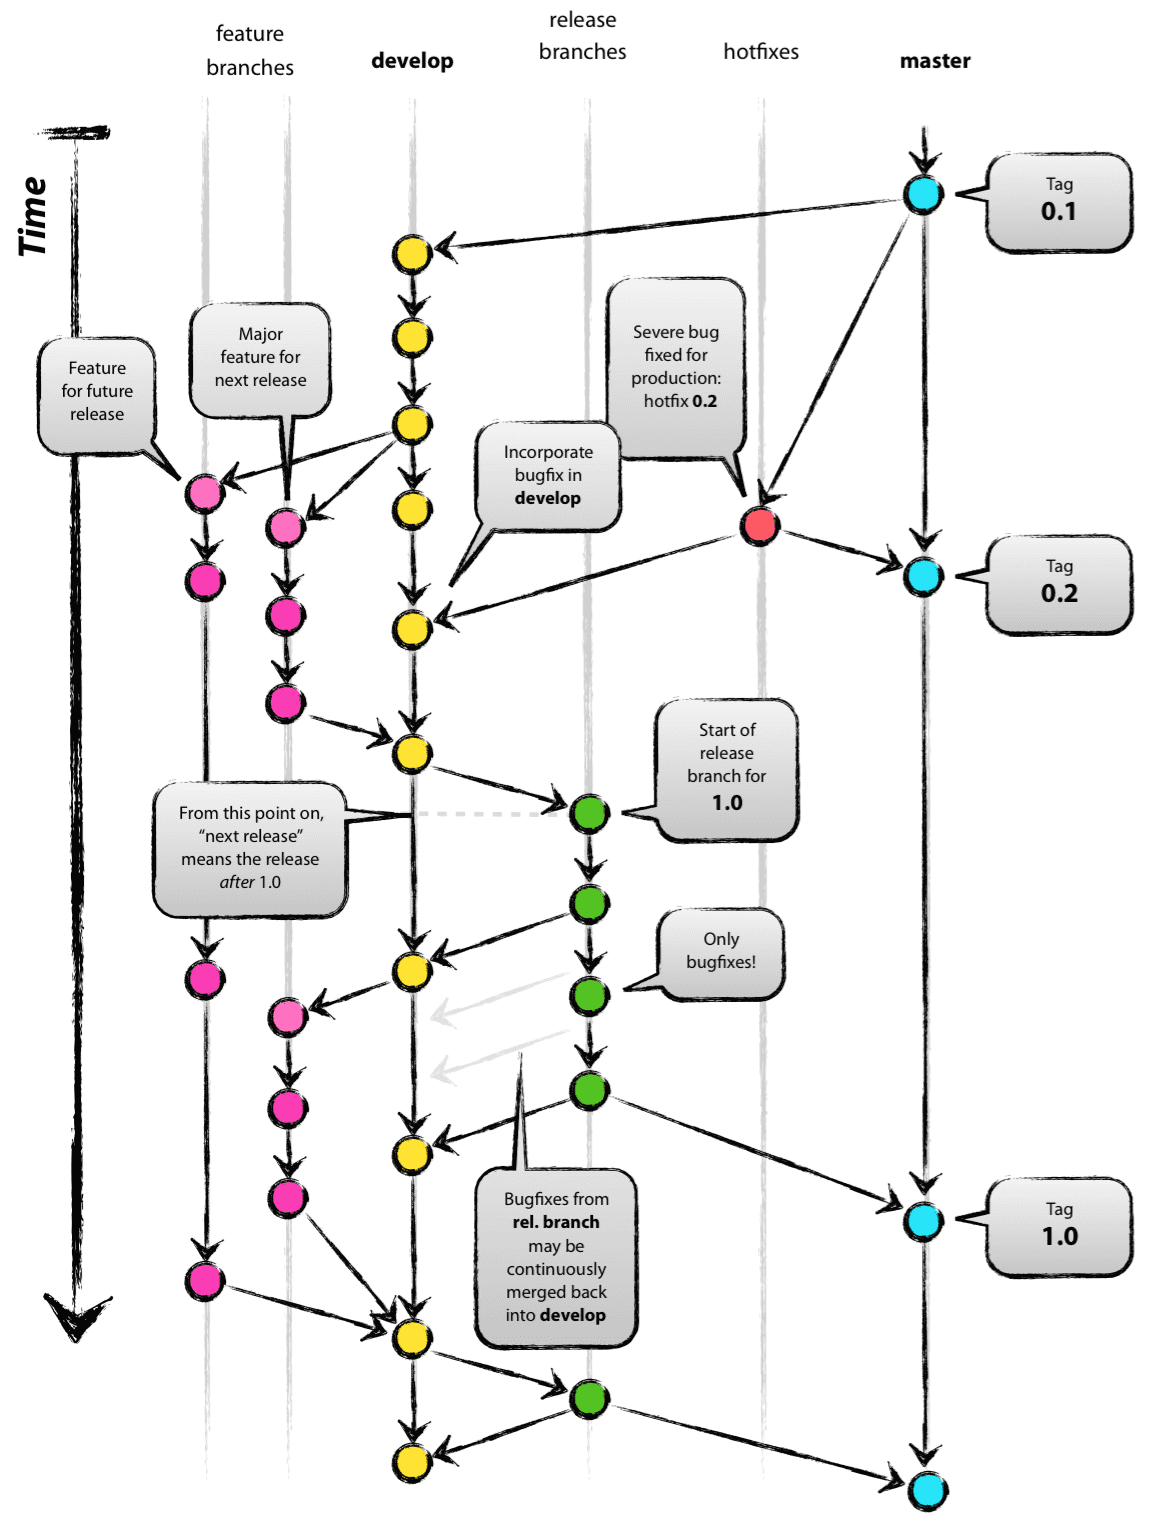
\includegraphics[width=0.55\linewidth]{estrategia}
 	\end{center}
 	\legend{Fonte: (http://nvie.com/posts/a-successful-git-branching-model/)}
 \end{figure}


\section{Os branches}

Na estratégia que iremos adotar vamos trabalhar com seis tipos de ramos, são eles, dois ramos principais e quatro tipos de ramos de apoio. 

Os ramos principais são os ramos \textit{master} e o \textit{develop}. E os ramos de apoio serão os ramos, \textit{feature}, \textit{release}, \textit{hotfix} e \textit{buxfix}. A seguir irei descrever cada um desses ramos. 

%Os ramos principais têm vida infinita, ou seja, eles sempre estarão presentes dentro do desenvolvimento, em contrapartida, os branches de apoio têm vida curta, sendo excluidos após suas utlizações, essas questões ficarão mais claras na prática.

\subsection{O \textit{branch} \textit{master}}

O ramo \textit{master} é o ramo que irá abrigar os códigos em suas versões mais estáveis. É o ramo que dará origem a aplicação final. Em algum momento do desenvolvimento todos os códigos produzidos em outros ramos farão um \textit{merge} (ato de mesclar os ramos, colocar os arquivos de um \textit{branch} em outro) com o \textit{branch master}, de forma direta ou indireta.

\subsection{O \textit{branch develop}}

Este ramo será responsável por conter os códigos em nível de desenvolvimento para o próximo \textit{deploy} (significa implementar, mas pode mudar de significado de acordo com o contexto). Lembre-se que os códigos não serão criados nesse \textit{branch}, esse é responsável apenas em abrigar os códigos que estão em desenvolvimento. Após os códigos serem devidamente testados, o \textit{branch develop} fará um merge com o \textit{branch master}, isso se nem um \textit{bug} for encontrado no processo de testes, esse processo está representado na figura \ref{develop}. Se o código aprensentar \textit{bug} será criado outro branch a partir do \textit{branch develop} para a correção dos \textit{bugs} e posteriormente mesclado com o \textit{branch master}.

\begin{figure}[H]
	\caption{\label{develop}O ramo \textit{develop}}
	\begin{center}
		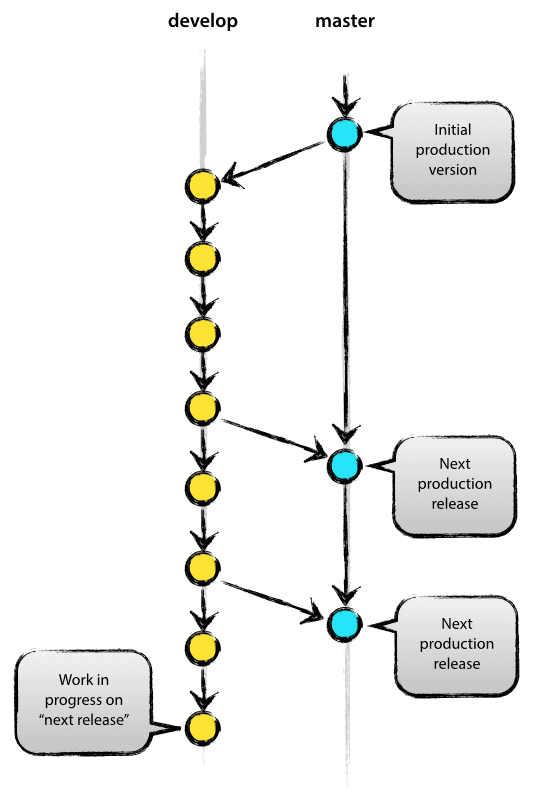
\includegraphics[width=0.3\linewidth]{develop}
	\end{center}
	\legend{Fonte: (http://nvie.com/posts/a-successful-git-branching-model/)}
\end{figure}
	
Os branches \textit{master} e \textit{develop}, possuem vida infinita, ou seja, eles sempre estarão presentes durante o desenvolvimento, e serão criados sempre que o git for inicializado. Os branches a seguir terão vida curta, eles serão criados e após suas utlizações eles serão finalizados e excluídos, esse processo firará mais claro na prática.

\subsection{O \textit{branch} \textit{feature}}

O branch feature representado na figura \ref{feature}, será utlizado sempre que uma nova funcionalidade precisar ser criada. Ele sempre será criado a partir do\textit{ branch develop} e finalizado no \textit{branch develop}, independente em qual ramo você esteja, isso se você estiver utlizando o \textit{git-flow}.

Ao contrário do ramo \textit{master} e \textit{develop}, o ramo \textit{feature} pode ser criado múltiplas vezes, uma para cada nova funcionalidade. Esse branch possui como prefixo \textit{feature/*}, onde o asterisco (*) será substituido pelo nome do "sub-ramo" \ digamos assim, por exemplo, \textit{feature/cadastrodeclientes}, \textit{feature/teladelogin}.

\begin{figure}[H]
	\caption{\label{feature}O ramo \textit{feature}}
	\begin{center}
		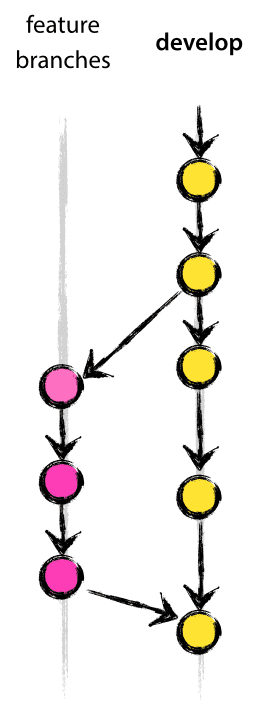
\includegraphics[width=0.2\linewidth]{feature}
	\end{center}
	\legend{Fonte: (http://nvie.com/posts/a-successful-git-branching-model/)}
\end{figure}


São duas as principais maneiras de mesclar branches, figura \ref{feature-merges}. A primeira é fazendo a mesclagem criando um novo \textit{commit} com as alterações dentro do ramo \textit{develop}, sem adicionar os \textit{commits} criados durante o desenvolvimento do ramo feature e, a outra é adicionando os \textit{commits} criados dentro do ramo feature dentro do ramo develop. Novamente, esse proceso ficará mais claro durante a prática.


\begin{figure}[H]
	\caption{\label{feature-merges}Tipos de merges}
	\begin{center}
		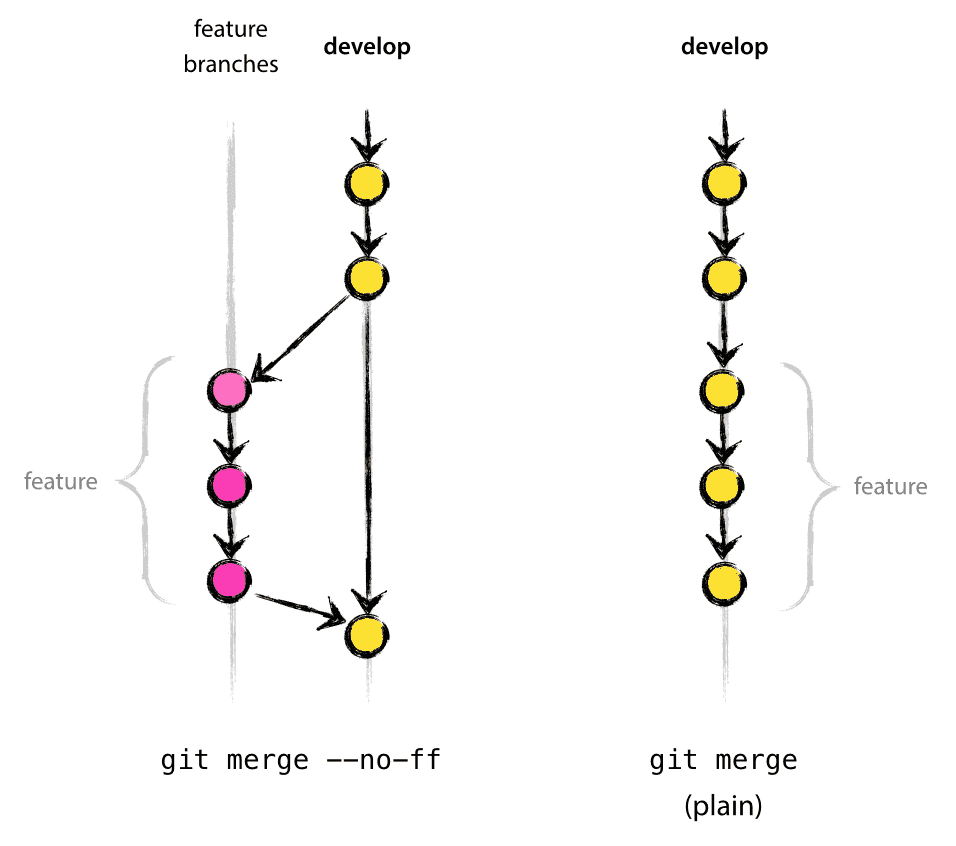
\includegraphics[width=0.6\linewidth]{feature-merges}
	\end{center}
	\legend{Fonte: (http://nvie.com/posts/a-successful-git-branching-model/)}
\end{figure}

\subsection{O \textit{branch release}}

Esse branch é o ramo intermediário entre o \textit{develop} e o \textit{master}. O objetivo desse branch é a criação de tags (são os números que indicam a versão da aplicação, 1.0.0, por exemplo). Ele inicia no branch develop e termina no \textit{branch master} e no \textit{develop}. Você deve está se perguntando porquê um branch que se inicia no develop tem que terminar no develop. Isso acontece porquê o \textit{branch} \textit{develop} tem que ter a mesma \textit{tag} do \textit{branch master}.


%%%%%%%%%%%%%%%%%%%%%%%%%%%%%%%%%%%%%%%%%%%%%%%%%%%%%%%%%%%%%%%%%%%%%%%%%
%\nocite{envelhecimento}
%\nocite{alice}
%\nocite{camarano}
%\nocite{constant}
%\nocite{karen}
%\nocite{secher}
%\nocite{Shimizu}
%\nocite{pompeo}
%\nocite{botelho}
%\nocite{moura}
%\nocite{trompieri}
%\nocite{anderson}
%\nocite{azevedo}
%\nocite{boer}
%\nocite{thomas}
%\nocite{shils}
%\nocite{raj}
%\nocite{kossioni}
%\nocite{eisele}
%\nocite{gille}
%\nocite{carvalho}
%\nocite{cancela}
%\nocite{philippi}
%\nocite{hordonho}
%\nocite{url1}
%\nocite{url2}
%\nocite{born}
%\nocite{costa}
%\nocite{heredia}
%\nocite{christophe}
%\nocite{garcia}
%\nocite{resende}
%\nocite{gois}
%\nocite{rezende}
%\nocite{perovano}
%
%\bibliography{biblio}
	 		
\end{document}
